\documentclass[letterpaper]{article}

\usepackage{aaai}
\usepackage{times}
\usepackage{helvet}
\usepackage{courier}
\usepackage{tikz}
\usetikzlibrary{arrows.meta, positioning}
\usepackage{courier}
\frenchspacing

\usepackage{amsthm}
\newtheorem{assumption}{Assumption}
\newtheorem{remark}{Remark}
\newtheorem{proposition}{Proposition}
\newtheorem{lemma}{Lemma}
\newtheorem{theorem}{Theorem}
 
\usepackage{amsmath, amssymb, bm}
\usepackage{booktabs}
\usepackage{etoolbox}
\usepackage[ruled,vlined,linesnumbered]{algorithm2e} 
\usepackage{xcolor}
\usepackage{comment}
\usepackage{tikz}
\usetikzlibrary{positioning, fit, backgrounds}
% Do NOT use geometry with aaai two-column style.
% \usepackage[margin=1in]{geometry}

% Make displayed equations smaller.
\AtBeginEnvironment{equation}{\small}
\AtBeginEnvironment{align}{\small}
\AtBeginEnvironment{align*}{\small}

% Compact displayed equations.
\setlength{\abovedisplayskip}{4pt}
\setlength{\belowdisplayskip}{4pt}
\setlength{\abovedisplayshortskip}{3pt}
\setlength{\belowdisplayshortskip}{3pt}

% Compact tables.
\newcommand{\tablesize}{\small}

\pdfinfo{
/Title (P-CONSENT: Committed Demand Response Backed by a Persistent, Negotiated EV Fleet)
/Author ()
}

\setcounter{secnumdepth}{0}

% ===================================================================
% Notation macros: change once, propagate everywhere.
% Indexed families take arguments, e.g. \soc{t}{v} -> \soc{t}{v}.
% ===================================================================
% --- Sets, indices, time
\newcommand{\Dset}{\mathcal{D}}              % days in billing cycle
\newcommand{\Tset}{\mathcal{T}}              % all time steps
\newcommand{\Td}{\mathcal{T}_{d}}              % steps of day d
\newcommand{\Tdv}{\mathcal{T}_{d}^{v}}           % steps of v's session on day d
\newcommand{\Vset}{\mathcal{V}}              % persistent users
\newcommand{\Vd}[1]{\mathcal{V}_{#1}}          % users with a session on day #1
\newcommand{\Kv}{\mathcal{K}_{v}}              % sessions of user v
\newcommand{\Tvk}{\mathcal{T}_{v,k}}           % steps of session k of user v
\newcommand{\dt}{\Delta t}                   % step length (h)
\newcommand{\evwin}[1]{\mathcal{T}^{\mathrm{DR}}_{#1}}         % DR event window of day #1
\newcommand{\tarr}{t_{\mathrm{arr}}}
\newcommand{\tdep}{t_{\mathrm{dep}}}
\newcommand{\treq}{t_{\mathrm{req}}}
% --- EVs, SoC, persistence
\newcommand{\soc}[2]{E_{#1}(#2)}             % SoC of #2 at time #1
\newcommand{\Earr}{E_{\mathrm{arr}}}
\newcommand{\Edep}{E_{\mathrm{dep}}}
\newcommand{\Ereq}{E_{\mathrm{req}}}
\newcommand{\Eneg}{E_{\mathrm{neg}}}
\newcommand{\Emin}{E_{\mathrm{min}}}
\newcommand{\Emax}{E_{\mathrm{max}}}
\newcommand{\wext}{w^{\mathrm{ext}}}          % external charging price
\newcommand{\Tpeak}{\mathcal{T}^{\mathrm{peak}}}
\newcommand{\pmax}{p^{\max}}
\newcommand{\pmaxpast}{p^{\max}_{\mathrm{past}}}
\newcommand{\assign}{\phi}                    % EV-to-charger assignment map
\newcommand{\pidr}{\pi^{\mathrm{DR}}}
\newcommand{\pich}{\pi^{\mathrm{ch}}}
\newcommand{\pineg}{\pi^{\mathrm{neg}}}
\newcommand{\Uflex}{U^{\mathrm{flex}}}
\newcommand{\Ubuf}{U^{\mathrm{buf}}}
\newcommand{\psihat}{\hat{\psi}}
\newcommand{\Pmaxhat}{\hat{P}_{\max}}
\newcommand{\Omeps}{\Omega_{\varepsilon}}
\newcommand{\State}{x}                       % system state
\newcommand{\Vfn}{V}                          % value function
\newcommand{\States}{\mathcal{S}}             % state space
\newcommand{\Acts}{\mathcal{A}}               % action space
\newcommand{\Kern}{\mathcal{P}}               % transition kernel
\newcommand{\Porc}{\mathcal{P}^{\star}}       % oracle problem
\newcommand{\Pdr}{\mathcal{P}^{\mathrm{DR}}}  % DR sub-problem
\newcommand{\Pch}{\mathcal{P}^{\mathrm{ch}}}  % charging sub-problem
\newcommand{\Pneg}{\mathcal{P}^{\mathrm{neg}}}% negotiation sub-problem
\newcommand{\Uexact}{U}                        % exact marginal value (oracle)
\newcommand{\zext}{\zeta^{\mathrm{ext}}}      % external charging cost to user
\newcommand{\Eext}{E_{\mathrm{ext}}}        % off-site (external) energy use
\newcommand{\banked}[2]{X(#1,#2)}            % banked excess at departure
\newcommand{\survived}[2]{S(#1,#2)}          % survived excess at arrival
\newcommand{\yieldf}[2]{\rho(#1,#2)}         % per-user yield
\newcommand{\accept}[2]{o(#1,#2)}            % over-charge acceptance
\newcommand{\buff}[1]{B_{#1}}                % realizable buffer of day #1
\newcommand{\buffhat}[1]{\hat{B}_{#1}}       % its day-ahead forecast
\newcommand{\ohat}{\hat{o}}                  % acceptance estimate
\newcommand{\rhohat}{\hat{\rho}}             % yield estimate
% --- Chargers, load, tariffs
\newcommand{\Nc}{N_{c}}
\newcommand{\rate}[2]{r_{#1}^{#2}}           % charging rate of #2 at #1
\newcommand{\rmin}[1]{r_{\min}^{#1}}
\newcommand{\rmax}[1]{r_{\max}^{#1}}
\newcommand{\avail}[2]{a_{#1}^{#2}}          % availability indicator
\newcommand{\Ptot}[1]{P_{#1}}                % total power draw
\newcommand{\bload}[1]{b_{#1}}               % non-EV building load
\newcommand{\we}[1]{w_{#1}^{e}}              % TOU energy price
\newcommand{\wdr}{w^{d}}                      % demand rate
\newcommand{\Kbatt}{K_{\mathrm{batt}}}
\newcommand{\Ksoc}{K_{\mathrm{SOC}}}
% --- Demand response
\newcommand{\FSL}{\mathrm{FSL}}
\newcommand{\Phist}{P^{\mathrm{hist}}}
\newcommand{\winc}{w^{\mathrm{inc}}}            % per-day capacity rate (tariff family w)
\newcommand{\Kfsl}{K_{\mathrm{FSL}}}
\newcommand{\vio}[1]{\sigma_{#1}}            % FSL violation slack
\newcommand{\Cinc}[1]{C_{#1}^{\mathrm{inc}}} % capacity payment
\newcommand{\Cpen}[1]{C_{#1}^{\mathrm{pen}}} % violation penalty
% --- Negotiation, payments, decisions
% --- Banking price, targets, guarantees (notation freeze) ---
\newcommand{\pbank}[2]{p^{\mathrm{bank}}_{#1,#2}}  % banking price for user #1, session #2 ($/kWh)
\newcommand{\cmarg}[1]{\hat{c}^{\,\mathrm{next}}_{#1}} % forecast next-session marginal supply cost
\newcommand{\DCmarg}{\Delta^{\mathrm{DC}}}          % demand-charge marginal of banking
\newcommand{\muDR}{\mu^{\mathrm{DR}}}               % event-value dual: $ per kWh of survived buffer
\newcommand{\etarget}[1]{E^{\mathrm{tgt}}_{#1}}     % terminal banking target of user #1 (kWh)
\newcommand{\Kbank}[1]{K^{\mathrm{bank}}_{#1}}      % terminal-shortfall reward weight of user #1
\newcommand{\Udc}{U^{\mathrm{dc}}}                  % demand-charge peak-share incentive
\newcommand{\pmaxre}{p^{\mathrm{re}}_{\max}}        % realized billing-cycle peak under replay
\newcommand{\bshort}[1]{\beta_{#1}}                 % banking shortfall of user #1 (kWh)
\newcommand{\Nexc}{N^{\star}}                       % exceedance-step count under optimized recourse
\newcommand{\Fsafe}{\FSL^{\mathrm{safe}}}           % demand-charge guardrail on the FSL
\newcommand{\epsIC}[2]{\varepsilon^{#1}_{#2}}       % IC slack of user #1 on day #2
\newcommand{\Umu}[1]{U(#1)}                  % marginal utility [CONSENT]
\newcommand{\gch}[2]{g_{#1}^{#2}}            % energy charged
\newcommand{\ucost}[2]{\zeta_{#1}^{#2}}      % user daily cost
\newcommand{\zund}[2]{z_{#1}^{#2}}           % unmet floor energy
\newcommand{\qdis}[2]{q_{#1}^{#2}}           % discharged energy
\newcommand{\act}[1]{A_{#1}}                 % charging action
 
\title{P-CONSENT: Committed Demand Response Backed by a Persistent, Negotiated Electric-Vehicle Fleet\\[4pt] {\large Paper Skeleton for Team Review}}

\author{}
\date{}

\begin{document}

\maketitle

\begin{abstract}
Commercial buildings can lower their electricity costs by committing ahead of time to demand response (DR) programs to shed their power draw during grid stress events, earning a capacity payment priced against a reduction below their usual peak known as a Firm Service Level (FSL), and incurring a penalty for any overshoot. Electric vehicles (EVs) parked at the workplace are a natural resource to back such a commitment, but they are not a reliable resource: they arrive and depart on their users' schedules, consume arbitrary amounts of charge to travel, and their available charge on any day depends on their off-site usage and past charging decisions. The building, therefore, commits usually a day ahead of an event, before the EVs that must satisfy the commitment have arrived. We present P-CONSENT, a framework that turns this persistent, self-interested fleet into a committed demand-response resource through three coordinated policies: (i) a day-ahead commitment policy that sizes the FSL against a forecast of the excess state of charge (SoC) buffer it expects to have, (ii) a real-time charging policy that banks charge across days to build that buffer and discharges it to hold the commitment, (iii) and a per-arrival negotiation policy that prices the excess SoC banking and flexibility, and settles payments only on what each vehicle's battery delivers. SoC Banking is priced so that it is free to the user exactly when the building needs the buffer, and never exploitable otherwise, and demand-response (DR) value reaches users only through their settled incentives, never as exposed program terms. We prove that the commitment satisfies a newsvendor-style optimality condition, that truthful reporting remains optimal up to a forecast error, that every payment is bounded by the value the user demonstrably creates, and that no participant is left worse off than charging elsewhere. Validated on operational data from a commercial building, the framework earns net demand-response revenue while lowering user charging costs and meeting its firm commitments.
\end{abstract}
%==============================================================
\section{Introduction} 

For commercial buildings, electricity costs are determined not only by total energy consumption but also by peak power: the demand charge, levied on the single highest power draw of a billing cycle, can account for over 30\% of the total bill \cite{neufeld1987demandcharge,neubauer2014demandcharge}.In addition, utilities operate demand response (DR) programs that provide a recurring capacity incentive to buildings that commit to a Firm Service Level (FSL), a limit on the power draw during grid stress events, and that impose penalties when the cap is violated during a called event~\cite{}. Traditionally, building operators curtail their electricity usage and physically turn off appliances to meet these curtailments~\cite{} which can cause inconvenience to the employees. In this work, we propose another avenue to achieve curtailment by leveraging the employee-owned electric vehicles (EVs) and charging facilities that commercial buildings typically have, incentivizing their use for building load management, while allowing users autonomy to refuse charging at the building. The growing presence of EVs at workplace facilities, along with bidirectional charging, is a resource suited to both objectives: a fleet of behind-the-meter batteries that can charge during low-price periods and discharge during peaks, reshaping the building's net load without curtailing building services~\cite{}. We show that by strategically negotiating with privately owned employee EVs having predictable, regular charging schedules at the building, a building operator can achieve lower monthly peaks (lower demand charges) and increase the FSL curtailment value, thereby increasing DR incentives and further reducing the building's electricity cost. The negotiations are targeted toward trading off a user's flexibility in state of charge (SoC) requirements and departure delays for monetary benefits.

Curtailment using the EVs, however, exposes a structural asymmetry between the building operator and the users. The capacity payment is earned by committing, a day or more in advance, to deliver load reduction during events whose timing the building does not control. Unlike a stationary battery, the EVs that help fulfil this commitment are intermittently available, since EVs arrive and depart according to their users' schedules, and are self-consuming. The energy stored in a vehicle may be expended in subsequent travel, with availability determined by charging decisions made on the preceding days \cite{iccps2026_pv2b}. Moreover, the EVs are owned by users who are self-interested and need to be well compensated for helping the building lower its bill. A building that commits to a lower, more aggressive FSL earns greater capacity revenue but bears the full delivery risk, and it needs to strategize and anticipate the user's behavior.
 
Resolving this asymmetry requires navigating a set of deeply interconnected challenges. First, the commitment is made under forecast uncertainty. The FSL must be committed before building loads, EV arrivals, and, critically, user cooperation for the day in question are realized, so the commitment is made against a forecast distribution rather than a realized schedule.  Second, the system must achieve incentive alignment without perfect user-side knowledge. Users must be compensated for flexibility in departure time and required SoC, and must not be able to profit by misreporting \cite{sen2026negotiations}. This is without any prior information available to the building about a user's preferences or a complete prediction of that user's behavior. Crucially, their negotiated SoC requirements must be met by departure. This leads to the third challenge of charging decisions. The charging actions need to balance the power use in high and low load times of the day. Moreover, the charge in EVs is temporally coupled. The energy buffer available for discharge on a high peak or a DR event day is the outcome of past charging decisions, off-site usage of the EVs, and the recurrence pattern of the EV. \cite{iccps2026_pv2b}. Single-day formulations, widely used in the EV charging literature, do not account for the temporal coupling across days, and the demand charge based on the monthly peak power defines sparse and delayed rewards.
 
Prior work addresses these challenges in isolation \textcolor{red}{(related-work section pending)}. Two-stage DR mechanism design \cite{satchidanandan2022two} formalizes the day-ahead-commitment, real-time-delivery structure, but for resources that are dispatchable and stationary rather than intermittently available, have private information, and are self-consuming. Strategy-proof daily negotiation \cite{sen2026negotiations} prices user flexibility and guarantees incentive compatibility, but it does not have temporal coupling across days, so that stored energy cannot be carried across day boundaries and the discharge depth available on a peak day is limited to the incidental surplus with which users arrive. Real-time V2B charging control with user persistence \cite{iccps2026_pv2b} handles the inter-day EV arrivals and charge planning, but it presumes complete cooperation from EV users and does not provide a structure for incentivizing. The reward is only for the long-horizon, sparse demand charge.  None of these approaches individually enables a building operator to provide a prior FSL commitment while requiring no prior commitment from its users.
 
We close this gap with P-CONSENT, a three-layer architecture with a deliberately asymmetric commitment structure. 
Layer~1, a day-ahead optimization between the building and the grid, determines the committed FSL. The commitment and its associated penalty are borne exclusively by the building. However, as shown later, the system tries to reduce the penalties by incorporating them in user negotiations. 
Layer~2, a negotiation mechanism using Monte-Carlo sampled model predictive control (MC-MPC), generates daily user options consistent with the previously fixed FSL. The layer compensates users for realized peak shaving and FSL penalty avoidance, with battery degradation incorporated into the payment. Users are negotiated with only at each arrival, with no future commitments required. 
Layer~3, another real-time Monte Carlo model predictive controller (MC-MPC) \cite{iccps2026_pv2b}, delivers against the committed FSL and the negotiated user requirements at minimum cost, using future samples and re-optimizing at fixed intervals, using updated building loads and EV status. On off-peak days, the controller over-charges consenting users above their negotiated SoC requirements, and is carried over to the subsequent day \cite{iccps2026_pv2b}. On high-peak or DR event days, it discharges the accumulated excess, along with smart planning for intra-day charge/discharge decisions.
Across the system, information flows unidirectionally, from the FSL commitment to the negotiation mechanism to the charging controller.
Our contributions are: 

\begin{itemize} 

\item \textbf{A formulation for DR participation backed by an intermittently available, self-consuming, temporally coupled resource (EVs) with private information}, with a three-layer decision structure whose within-day information flow is unidirectional (from the FSL commitment to the negotiation mechanism to the charging controller) and whose cross-day loop closes through the persistent SoC buffer.
% (Section~\ref{sec:formulation}). 

% \item \textbf{A characterization of the feasible commitment set}, establishing that the set of FSLs deliverable at a given risk level grows monotonically with the forecast buffer, thereby formalizing the manner in which persistence-aware over-charging expands upstream commitment capacity (Proposition~\ref{prop:monotone}), together with a commitment-depth parameter that prices the building's delivery risk and a newsvendor-type characterization of the risk-neutral optimal commitment, which anchors the depth parameter to a principled operating point. 

\item \textbf{A rigorous user negotiation mechanism} where user offers are weakly strategy-proof, incentive compatible and allow voluntary participation.
% we state precisely which of CONSENT's guarantees transfer unchanged and which require restatement under the over-charge policy (Section~4). 

\item \textbf{An evaluation on real building, tariff, and EV fleet data} from a commercial facility (Nissan Advanced Technology Center, Silicon Valley), demonstrating that the combined architecture weakly dominates building-only, negotiation-only, and persistence-only baselines with respect to both building and user cost, with sensitivity analyses over the cost-sharing parameter $\alpha$ \cite{sen2026negotiations} and the commitment depth (Section~\ref{sec:eval}). 

\end{itemize}

% Three-policy-lane view of P-CONSENT. The three policies are the primary
% structure: pi^DR (day-ahead), pi^ch (every dt), pi^neg (per arrival), each
% on its own clock. Vertical arrows are the within-day dependency (FSL ->
% charging feasible set -> negotiation options); the dashed arrow is the sole
% cross-day link (surviving buffer). Not a timeline: see Sec. 4.
% Requires \usetikzlibrary{positioning, fit, backgrounds, arrows.meta}.
\begin{figure*}[t]
\centering
\newcommand{\ltitle}{\bfseries}%
\newcommand{\leqn}{\scriptsize\itshape\color{black!55}}%
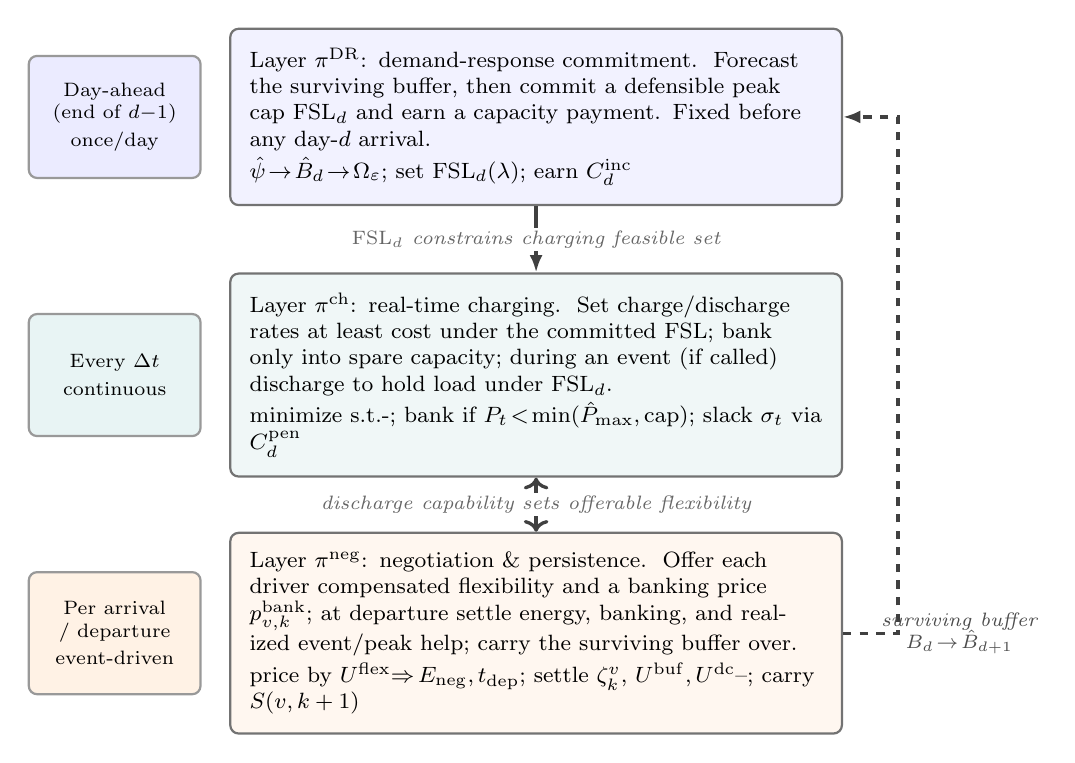
\begin{tikzpicture}[
  font=\footnotesize,
  every node/.style={transform shape},
  lane/.style={rectangle, rounded corners=3pt, draw=black!55, thick,
               align=left, inner sep=7pt, text width=0.60\textwidth,
               minimum height=1.55cm},
  clock/.style={rectangle, rounded corners=3pt, draw=black!40, thick,
                fill=white, align=center, inner sep=4pt, text width=1.9cm,
                minimum height=1.55cm, font=\scriptsize},
  dep/.style={-{Latex[length=2.2mm]}, very thick, black!75},
  back/.style={-{Latex[length=2.2mm]}, very thick, dashed, black!75},
  deplab/.style={font=\scriptsize\itshape, text=black!60, align=center, fill=white, inner sep=1pt}
]
% ============ LANE 1: pi^DR (day-ahead) ============
\node[clock, fill=blue!8] (cDR) {\ltitle Day-ahead\\(end of $d{-}1$)\\[2pt]\leqn once/day};
\node[lane, fill=blue!5, right=0.35cm of cDR] (DR) {%
{\ltitle Layer $\pidr$: demand-response commitment.}\ \ Forecast the surviving
buffer, then commit a defensible peak cap $\FSL_d$ and earn a capacity payment.
Fixed before any day-$d$ arrival.\\[2pt]
{\leqn $\psihat\!\to\!\buffhat{d}\!\to\!\Omeps$; set
$\FSL_d(\lambda)$;\ earn $\Cinc{d}$}};

% ============ LANE 2: pi^ch (every dt) ============
\node[clock, fill=teal!9, below=1.7cm of cDR] (cCH) {\ltitle Every $\dt$\\[2pt]\leqn continuous};
\node[lane, fill=teal!6, right=0.35cm of cCH] (CH) {%
{\ltitle Layer $\pich$: real-time charging.}\ \ Set charge/discharge rates at
least cost under the committed FSL; bank only into spare capacity; during an
event (if called) discharge to hold load under $\FSL_d$.\\[2pt]
{\leqn minimize s.t.\--;
bank if $\Ptot{t}\!<\!\min(\Pmaxhat,\text{cap})$; slack $\vio{t}$ via $\Cpen{d}$}};

% ============ LANE 3: pi^neg (per arrival) ============
\node[clock, fill=orange!10, below=1.7cm of cCH] (cNEG) {\ltitle Per arrival\\/ departure\\[2pt]\leqn event-driven};
\node[lane, fill=orange!6, right=0.35cm of cNEG] (NEG) {%
{\ltitle Layer $\pineg$: negotiation \& persistence.}\ \ Offer each driver
compensated flexibility and a banking price $\pbank{v}{k}$; at departure settle
energy, banking, and realized event/peak help; carry the surviving buffer over.\\[2pt]
{\leqn price by $\Uflex$$\Rightarrow\!\Eneg,\tdep$; settle
$\ucost{k}{v}$, $\Ubuf,\Udc$--;
carry $\survived{v}{k+1}$}};

% ============ WITHIN-DAY DEPENDENCY (top -> down) ============
\draw[dep] (DR.south) -- (CH.north)
  node[deplab, midway] {$\FSL_d$ constrains charging feasible set};
\draw[dep, <->] (CH.south) -- (NEG.north)
  node[deplab, midway] {discharge capability sets offerable flexibility};

% ============ CROSS-DAY LINK (bottom -> up, dashed) ============
\draw[back] (NEG.east) -- ++(0.7,0)
  node[midway, right, font=\scriptsize\itshape, text=black!70, align=center]
    {surviving buffer\\ $\buff{d}\!\to\!\buffhat{d+1}$}
  |- (DR.east);

  

\end{tikzpicture}
\caption{The three policies of P-CONSENT, each acting on its own clock:
$\pidr$ commits the firm service level a day ahead, $\pich$ sets charging and
discharging rates every $\dt$, and $\pineg$ negotiates flexibility and settles
payments at each arrival and departure. Solid vertical arrows are the sole
within-day dependency, the committed FSL constrains the charging feasible set,
which in turn sets the flexibility the negotiation can offer; this is a
dependency, not a temporal order, since the charging and negotiation epochs
interleave continuously through the day (the problem definition (Section~\ref{sec:formulation})). The dashed
arrow is the only coupling between days: the buffer that survives a driver's
trip becomes tomorrow's deliverable buffer and sharpens the forecast that sets
the next commitment.}
\label{fig:processflow}
\end{figure*}


%==============================================================
\section{Problem Definition (Outline)}\label{sec:formulation}

\paragraph{Setting.} A commercial building hosts workplace EV charging for
a population of \emph{returning} commuters. Its bill has three components:
time-of-use energy, a monthly demand charge $\wdr{}\,\pmax$ on the single
highest power draw of the billing cycle, and a demand-response layer
(PG\&E Capacity Bidding Program): the building commits a Firm Service
Level $\FSL_d$ at the end of day $d{-}1$, earns $\winc$ per kW the
commitment sits below its baseline, and pays $\Kfsl$ per kWh drawn above
it during a called event window. The commitment is made roughly 30 hours
before an afternoon event, before the fleet that must satisfy it has
arrived.

\paragraph{Three coupled sub-problems.} We decompose the operator's
problem into three policies, each on its own clock
(Figure~\ref{fig:processflow}):
\begin{itemize}
\item $\pidr$ (\emph{day-ahead}): choose $\FSL_d$ against a forecast of
the surviving buffer, via an $\varepsilon$-feasible commitment set and a
depth parameter $\lambda$ interpolating from the null commitment to the
deepest defensible one.
\item $\pich$ (\emph{every $\dt$}): set charge/discharge rates at least
cost under the committed FSL; bank charge into headroom toward a
per-user terminal target $\etarget{v}$ so banking never creates a new
peak; discharge during events to hold the cap.
\item $\pineg$ (\emph{per arrival/departure}): offer each driver
compensated flexibility options and a banking price $\pbank{v}{k}$;
settle at departure on realized quantities only.
\end{itemize}

% Stage-1 commitment optimizes by simulating Stage-2 recourse over sampled
% populations: users enter first as model draws, then as real arrivals.
% Single-column figure for the approach section.
\begin{figure}[t]
\centering
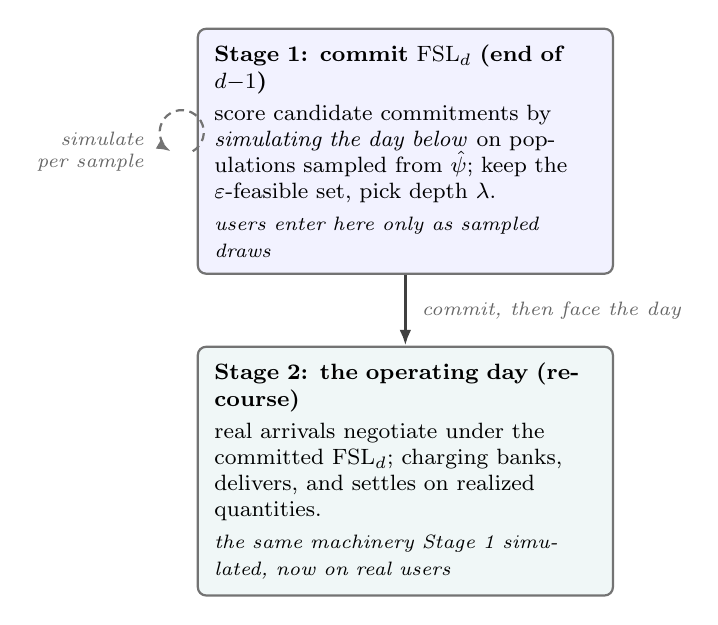
\begin{tikzpicture}[
  font=\footnotesize,
  every node/.style={transform shape},
  stg/.style={rectangle, rounded corners=3pt, draw=black!55, thick,
              align=left, inner sep=6pt, text width=0.40\textwidth},
  dep/.style={-{Latex[length=2mm]}, very thick, black!75},
  lo/.style={-{Latex[length=1.8mm]}, thick, black!55, densely dashed}
]
\node[stg, fill=blue!5] (s1) {%
{\bfseries Stage 1: commit $\FSL_d$ (end of $d{-}1$)}\\[2pt]
score candidate commitments by \emph{simulating the day below} on
populations sampled from $\psihat$; keep the $\varepsilon$-feasible set,
pick depth $\lambda$.\\[2pt]
{\scriptsize\itshape users enter here only as sampled draws}};

\node[stg, fill=teal!6, below=0.9cm of s1] (s2) {%
{\bfseries Stage 2: the operating day (recourse)}\\[2pt]
real arrivals negotiate under the committed $\FSL_d$; charging banks,
delivers, and settles on realized quantities.\\[2pt]
{\scriptsize\itshape the same machinery Stage 1 simulated, now on real users}};

\draw[dep] (s1) -- (s2) node[midway, right=2pt, font=\scriptsize\itshape, text=black!60]{commit, then face the day};

\draw[lo] (s1.west) ++(-0.05,0) arc[start angle=-60, end angle=240, radius=0.28]
  node[left=6pt, font=\scriptsize\itshape, text=black!60, align=right]{simulate\\per sample};
\end{tikzpicture}
\caption{The commitment is chosen by rehearsing its own consequences: Stage 1
scores each candidate $\FSL_d$ by running the Stage-2 negotiation and
charging machinery on populations sampled from the forecast, then commits;
on the day itself the identical machinery runs on the real arrivals. Users
appear twice, first as model draws inside the rehearsal, then as arriving
negotiators, which is what makes the commitment feasible before its
resource exists.}
\label{fig:twostage}
\end{figure}


\paragraph{Persistence.} A user's arrival SoC couples to their prior
departure, $\Earr = \Edep - \Eext$; excess banked on one visit, less
off-site use, survives as $\survived{v}{k+1}$ and aggregates into the
deliverable buffer $\buff{d}$. Persistence is both the complication
(single-day formulations cannot represent it) and the resource (the
buffer is what backs an aggressive commitment).

\paragraph{The money.} All transfers are inside one objective. The user
pays energy and a banking settlement $\pbank{v}{k}\banked{v}{k}$; the
building pays a flexibility incentive $\alpha\Uflex$, and two ex-post
replay incentives that partition one realized saving: $\Ubuf$
(event-penalty share) and $\Udc$ (demand-charge share). The banking
price is constructed so banked energy is free exactly when the building
wants the buffer (pre-event, via the event-value dual $\muDR$) and
arbitrage-neutral otherwise. Users never see program terms; DR value
reaches them only through settled incentives.

\paragraph{The coupled problem.} Jointly, this is a semi-Markov decision
process with three epoch types (day-boundary, control, arrival) that
\emph{interleave}; the only within-day dependency is one-way
($\FSL_d \to$ charging feasible set $\to$ negotiation options) and the
only cross-day coupling is the surviving buffer and the running peak. A
perfect-information oracle over the billing cycle provides the lower
bound; the deployed system differs from it only in information and
decomposition, not in the objective.

%==============================================================
\section{Proposed Guarantees (Outline)}\label{sec:guarantees-outline}

Each guarantee below is stated informally with the mechanism that
achieves it; formal statements and proofs are drafted (full versions in
the working manuscript).

\begin{itemize}
\item \textbf{Periodic ex-post incentive compatibility, up to forecast
error} (Thm.~1). No user can gain more than
$\epsIC{v}{d}$ by misreporting departure time or required SoC, on any
day, for any realization of others.
\emph{Intuition:} misreports only shrink the feasible set of the
charging problem, so the marginal utility that prices a user's options
can only fall (a set-inclusion argument that survives any change of
objective, including the DR terms); the one residual channel, banking
arbitrage, is closed by pricing banked energy at the maximum of today's
cost and the forecast next-day cost, leaving a gap bounded by forecast
error. The banked amount itself is a controller decision, so it is not
reportable. This is the strongest strategy-proofness attainable in
this setting: dominant-strategy IC is structurally unavailable once a
user's private valuation evolves across sessions.
\item \textbf{Budget feasibility} (Thm.~2 + Lemma~1). Every payment is
bounded by value the user demonstrably creates: flexibility payments by
a telescoping sum of sequential marginals; the replay incentives
$\Ubuf + \Udc$ by a proportional-share cap against the single realized
replay saving they partition.
\emph{Intuition:} paying capped marginals of one realized number cannot
exceed that number; the partition (rather than two independent solves)
is what makes double counting impossible.
\item \textbf{Voluntary participation.} Every session, the user can
reject all offers and charge externally at $\wext$; banking is opt-in;
event days only improve offered terms. No participant is ever worse off
than their outside option.
\item \textbf{Newsvendor characterization of the commitment}
(Prop.~2). (\emph{Newsvendor}: the classical inventory model of committing a quantity before uncertainty realizes, balancing a certain per-unit gain against an expected per-unit shortfall cost.) The risk-neutral optimal FSL equates the certain per-kW
capacity rate with the expected marginal penalty over event-window
exceedance steps, $\winc = \Kfsl\,\dt\,\mathbb{E}[\Nexc]$.
\emph{Intuition:} lowering the cap by 1\,kW earns $\winc$ for sure and
risks $\Kfsl$ per exceedance step; the optimum balances them.
\emph{Regime finding (empirical, micro-scale):} at actual CBP rates the
risk-neutral point is \emph{deeper} than any $\varepsilon$-feasible
commitment, so the risk floor binds ($\lambda^{\star}$ clamps to 1) and
the deployed range $\lambda < 1$ is priced risk aversion; the interior
regime appears when the penalty dominates. The risk overlay is
load-bearing at program rates, which we will characterize by sweeping
$\winc$ across the regime boundary.
\item \textbf{Monotonicity of the commitment set.}
\begin{proposition}[informal]\label{prop:monotone}
A larger surviving buffer weakly deepens the feasible commitment and
weakly raises attainable capacity revenue.
\end{proposition}
\emph{Intuition:} more dischargeable energy only relaxes the
event-window delivery constraint, scenario by scenario.
\item \textbf{Conditional temporal decomposition} (Thm.~3). Within the
policy class of per-day policies plus a scalar terminal banking target
per user, the billing-cycle problem separates by day; the price is a
certainty-equivalence gap that vanishes under exact forecasts and is
reported empirically.
\item \textbf{Demand-charge guardrail} (Prop.~3). An explicit level
$\Fsafe$ below which a commitment can conflict with the monthly peak;
above it the conflict is impossible, deterministically.
\end{itemize}

\noindent\textbf{Status.} All mechanisms above are implemented in our
simulator and verified on micro-instances (partition exactness,
free-riding exploit closed by the banking price, ledger caps binding
only in constructed complementary cases, carryover exact, newsvendor
condition reproduced unconstrained). What remains is the full-scale
experimental campaign below.


%==============================================================
\section{Notation Summary}\label{sec:notation}

\begin{table*}[t]
\centering\small
\caption{Principal symbols, grouped by layer. ``Set by'' names the deciding
party or process.}
\label{tab:skeleton-notation}
\begin{tabular}{@{}p{0.22\textwidth}p{0.42\textwidth}p{0.24\textwidth}@{}}
\toprule
Symbol & Meaning & Set by \\
\midrule
\multicolumn{3}{@{}l}{\emph{Commitment layer}} \\
$\FSL_d$ & committed power cap, day $d$ & $\pidr$, day-ahead \\
$\winc$, $\Kfsl$ & capacity rate; overshoot penalty & tariff \\
$\vio{t}$ & FSL violation slack & realized \\
$\Omeps$, $\lambda$, $\varepsilon$ & feasible set; depth; risk level & SAA; operator \\
$\Nexc$, $\Fsafe$ & exceedance count; guardrail & derived \\
\midrule
\multicolumn{3}{@{}l}{\emph{Billing}} \\
$\we{t}$, $\wdr{}$ & TOU price; demand rate & tariff \\
$\pmax$, $\pmaxpast$ & cycle peak; running peak & realized \\
\midrule
\multicolumn{3}{@{}l}{\emph{Persistence and banking}} \\
$\banked{v}{k}$, $\Eext$ & banked excess; off-site use & $\pich$; user \\
$\survived{v}{k}$, $\yieldf{v}{k}$ & survived excess; yield & realized \\
$\accept{v}{k}$, $\buff{d}$, $\buffhat{d}$ & consent; buffer; forecast & user; realized; $\pidr$ \\
$\etarget{v}$, $\Kbank{v}$, $\bshort{v}$ & bank target; weight; shortfall & $\pidr \to \pich$ \\
\midrule
\multicolumn{3}{@{}l}{\emph{Prices and payments}} \\
$\pbank{v}{k}$ & banking price on excess & mechanism \\
$\cmarg{v}$, $\DCmarg$, $\muDR$ & next-cost forecast; DC marginal; event dual & forecast; $\pich$; dual \\
$\Uflex$, $\alpha$ & flexibility value; cost share & mechanism; operator \\
$\Ubuf$, $\Udc$ & replay shares: penalty; demand & ex-post replay \\
$\ucost{k}{v}$, $\wext$ & session cost; external rate (IR floor) & settlement; market \\
$\epsIC{v}{d}$ & IC slack bound & forecast error \\
\bottomrule
\end{tabular}
\end{table*}

Table~\ref{tab:skeleton-notation} collects the symbols used above; the full
manuscript carries the complete tagged variable tree.

%==============================================================
\section{Experiment Plan}\label{sec:expplan}

Data: operational building load and charging telemetry from a commercial
site (May~2023--Nov.~2024), utility TOU tariffs, CBP rates
($\winc{=}\$13.6$/kW, $\Kfsl{=}\$6$/kWh). 50 test episodes/month over 8
months, $\geq 5$ seeds, paired bootstrap CIs on all headline deltas,
common random numbers across counterfactuals, config-hash provenance on
every result.

\paragraph{Claims and their experiments.}
\begin{itemize}
\item \textbf{C1 (headline):} the full system earns net DR revenue at
equal or better user cost than the best non-committing baseline.
\emph{Main table} over a baseline ladder: building-only; uncoordinated;
smart charging; single-day negotiation (CONSENT); persistence banking
without negotiation (P-V2B); negotiation with naive bolt-on DR;
operator-controlled banking with DR but no mechanism; \textbf{P-CONSENT};
perfect-information oracle. Metrics: net building cost, DR revenue and
penalty, user \$/kWh, reject rate, FSL delivery rate, missing SoC,
battery throughput.
\item \textbf{C2 (causality):} banking causally expands the safely
committable FSL. Sweep the banking reward $\Kbank{v}$ (not the buffer by
fiat, so the causal path runs through dispatch); report
$\min\Omeps$, realized FSL, revenue; report any monotonicity violations
at charger-capacity kinks honestly.
\item \textbf{C3 (commitment):} the $(\lambda,\varepsilon)$ frontier and
the regime boundary. Frontier sweep $\lambda \times \varepsilon$
(revenue, penalty, delivery rate); \emph{regime sweep of $\winc$} across
the boundary where $\lambda^{\star}$ moves from interior to clamped;
verify the unconstrained newsvendor condition
$\mathbb{E}[\Nexc(\FSL^{\star})] = \winc/(\Kfsl\dt)$ on the value curve.
\item \textbf{C4 (incentives):} empirical $\varepsilon$-IC. Deviation
harness over all users and episodes (earlier departures, inflated SoC);
violation CDF against the bound, split event vs.\ non-event days; the
free-riding exploit shown profitable with the banking price disabled and
closed with it enabled.
\item \textbf{C5 (ledger):} per-day budget feasibility audit including
the replay caps; a constructed complementary-buffer day showing the cap
binding.
\item \textbf{C6 (decomposition):} certainty-equivalence gap of the
target-coupled per-day solution vs.\ a joint two-day solve on
downsampled instances; gap $\to$ 0 under a degenerate forecast.
\item \textbf{C7 (robustness):} value vs.\ yield $\rho$ and acceptance
$o$ (heatmap with break-even contour); forecast-degradation sweep;
scenario-count sensitivity.
\item \textbf{C8 (guardrail):} realized monthly peaks with commitments
above vs.\ (forced) below $\Fsafe$; zero new-peak events above it.
\end{itemize}

\paragraph{Ablations.} One row per removed component: banking price off
(exploit turns profitable), terminal target off ($K^{\mathrm{bank}}{=}  0$,
banking degenerates to tie-breaking), replay settlement replaced by
ex-ante incentive share (funding overdraw reappears), peak-share $\Udc$
off (non-event peak value unpaid), reject-all off, guardrail off. Each
row: building cost, user cost, penalty, delivery rate, exploit
profitability.

\paragraph{Deliverables.} Three main tables (results ladder; sensitivity
across user-flexibility profiles and cost-share $\alpha$; ablations) and
five main figures (architecture; $(\lambda,\varepsilon)$ frontier with
the regime boundary; $(\rho,o)$ heatmap; $\varepsilon$-IC violation CDF
vs.\ bound; runtime scaling), remainder to appendix. Priority under
deadline pressure: main table, frontier + regime sweep, heatmap,
$\varepsilon$-IC, ablations first; all else second.

%==============================================================
\bibliographystyle{aaai}
\bibliography{references}

\end{document}
